\documentclass{sigchi}
\usepackage{autobreak}
\newcommand\tabhead[1]{\small\textbf{#1}}
\makeatletter
\def\@copyrightspace{\relax}
\makeatother


% Use this command to override the default ACM copyright statement (e.g. for preprints). 
% Consult the conference website for the camera-ready copyright statement.


%% EXAMPLE BEGIN -- HOW TO OVERRIDE THE DEFAULT COPYRIGHT STRIP -- (July 22, 2013 - Paul Baumann)
% \toappear{Permission to make digital or hard copies of all or part of this work for personal or classroom use is 	granted without fee provided that copies are not made or distributed for profit or commercial advantage and that copies bear this notice and the full citation on the first page. Copyrights for components of this work owned by others than ACM must be honored. Abstracting with credit is permitted. To copy otherwise, or republish, to post on servers or to redistribute to lists, requires prior specific permission and/or a fee. Request permissions from permissions@acm.org. \\
% {\emph{CHI'14}}, April 26--May 1, 2014, Toronto, Canada. \\
% Copyright \copyright~2014 ACM ISBN/14/04...\$15.00. \\
% DOI string from ACM form confirmation}
%% EXAMPLE END -- HOW TO OVERRIDE THE DEFAULT COPYRIGHT STRIP -- (July 22, 2013 - Paul Baumann)


% Arabic page numbers for submission. 
% Remove this line to eliminate page numbers for the camera ready copy
% \pagenumbering{arabic}


% Load basic packages
\usepackage{balance}  % to better equalize the last page
\usepackage{graphics} % for EPS, load graphicx instead
\usepackage{times}    % comment if you want LaTeX's default font
\usepackage{url}      % llt: nicely formatted URLs

% llt: Define a global style for URLs, rather that the default one
\makeatletter
\def\url@leostyle{%
  \@ifundefined{selectfont}{\def\UrlFont{\sf}}{\def\UrlFont{\small\bf\ttfamily}}}
\makeatother
\urlstyle{leo}


% To make various LaTeX processors do the right thing with page size.
\def\pprw{8.5in}
\def\pprh{11in}
\special{papersize=\pprw,\pprh}
\setlength{\paperwidth}{\pprw}
\setlength{\paperheight}{\pprh}
\setlength{\pdfpagewidth}{\pprw}
\setlength{\pdfpageheight}{\pprh}

% Make sure hyperref comes last of your loaded packages, 
% to give it a fighting chance of not being over-written, 
% since its job is to redefine many LaTeX commands.
\usepackage[pdftex]{hyperref}
\hypersetup{
pdftitle={Research on indoor positioning technology based on iBeacon},
pdfauthor={Shanliang Yao},
pdfkeywords={indoor positioning, iBeacon, Triangle Algorithm, Weighted Trilateration Algorithm},
bookmarksnumbered,
pdfstartview={FitH},
colorlinks,
citecolor=black,
filecolor=black,
linkcolor=black,
urlcolor=black,
breaklinks=true,
}

% create a shortcut to typeset table headings
\newcommand\tabhead[1]{\small\textbf{#1}}


% End of preamble. Here it comes the document.
\begin{document}

\title{Research on indoor positioning technology based on iBeacon}

\numberofauthors{1}
\author{
  \alignauthor Shanliang Yao\\
    \affaddr{Xi'an Jiaotong Liverpool University}\\
    \email{shanliang.yao19@student.xjtlu.edu.cn}\\
    \affaddr{+86 18896581232}
}

\maketitle

\begin{abstract}
Nowadays, some specific locations have troubled people when they look for their destinations. For example, when people are in an unfamiliar underground garage, people may get trapped when looking for their cars because there is no GPS signal. The practicability and necessity of indoor positioning in some specific occasions have become increasingly significant.

iBeacon is a new type of precision indoor micro-positioning technology based on Bluetooth 4.0. Currently, iOS and Android system devices all have Bluetooth Low Energy Technology (BLE) \cite{gomez2012overview}. In practice, there are multiple algorithms to obtain an accurate position. In this research, the researcher will compare Trilateration Algorithm to Weighted Trilateration Algorithm and analyze the experiment data after several experiments. The research will be done under the hypothesis that Weighted Trilateration Algorithm outweighs Trilateration Algorithm in its stability and accuracy which can help people reach their destinations. 

\textbf{keywords}: indoor positioning, iBeacon, Triangle Algorithm, Weighted Trilateration Algorithm
\end{abstract}

\section{Introduction}

Numerous mobile applications (APP) are currently making use of positioning technologies such as the Global Positioning System (GPS) \cite{misra2006global}, which could detect the position information of the users. However, due to the signal attenuation caused by the construction materials of buildings or undergrounds, positioning systems cannot rely on the GPS.

Bluetooth is a wireless technology standard for exchanging data over short distances. Also, it has been used for indoor localization since it is a cost-effective and easy-to-deploy solution. With the progress and development of telecommunication technologies, a recently proposed technology called iBeacon is widely adapted in many applications.

iBeacon is an emerging technology in the field of indoor positioning that has shown better performance compared to others. It is a set of protocols that can be used in indoor positioning systems by Apple. The protocols indicate that a new low-power, low-cost signal transmitter can be detected by nearby handheld electronic devices. When your device is close to an iBeacon base station, the device can sense the iBeacon signal (UUID and RSSI) \cite{feldmann2003indoor}, ranging from a few millimeters to 50 meters. This technology allows smartphones or other devices to execute commands within the sensing range of an iBeacon base station.


\section{Literature Review}

This chapter first reviews different technologies in the field of indoor positioning. Then, it elaborates on the iBeacon technology. After that, it studies some algorithms about the indoor position. And finally, by summarizing all, it identifies and pins down some key issues that need to be addressed in the present study.

\subsection{Indoor Positioning Technology}

Indoor positioning has emerged as a critical function in many applications: including indoor personnel guidance, equipment guidance, security monitoring, property security and smart factories. From the journal \emph{Global Positioning System: signals, measurements and performance second edition} \cite{alarifi2016ultra}, it tell us that in comparison with outdoor environments, sensing location information in indoor environments requires a higher precision and is a more challenging task in part because various objects reflect and disperse signals . 

Technologies of indoor positioning vary, like Radio Frequency Identification (RFID), Ultra Wideband (UWB), Infrared (IR), Ultrasonic, Zigbee, Wireless Local Area Network (WLAN), Cellular Based, Bluetooth \cite{mautz2012indoor}. 

\subsection{iBeacon Technology}

In the World Wide Developers Conference (WWDC) 2013 event, Apple announced iBeacon, a technology that enables a device (called beacon) to send push notifications to nearby iOS devices \cite{conte2014bluesentinel}. The iBeacon is Apple's implementation of BLE wireless technology to create a different way of providing location-based information services to mobile devices. It acts as an emitter continuously broadcasting Bluetooth signals, in which each signal contains a Universally Unique Identifier (UUID) and a Received Signal Strength Indicator (RSSI).

This technology has significant advantages compared to other types of indoor positioning technologies, in its less expensive hardware, less energy consumption, needless to the internet connection, and is capable of receiving notifications in the background. This technology will provide huge benefits for future location awareness applications. It will change the way retailers, event organizers, and educational institutions communicate with people indoors \cite{fard2015indoor}. 


\subsection{Indoor Positioning Algorithms}

At present, there are various indoor positioning algorithms on the market which based on the principle of acquiring the signal strength of the surrounding Bluetooth base station through phones or other devices, such as Kalman Filter Algorithm, Gaussian Filtering Algorithm, Trilateration Algorithm and Weighted Trilateration Algorithm. In this research, I select Weighted Trilateration Algorithm and conduct experiments to compare it with the Trilateration Algorithm as both of them are the excellent algorithms and need to be researched more to discover the differences.

\subsubsection{Trilateration Algorithm}

In the ranging-based positioning algorithm, the Trilateration Algorithm \cite{liu2018trilateration} is a basic algorithm. The algorithm principle is: there are three non-collinear base stations A, B, C, and an unknown device D on the plane. The distance from the base station to the device D is R1, R2, and R3, and the coordinates of the three base stations are the center of the circle. The distance from the three base stations to the unknown device can be drawn as three intersecting circles, as shown in the following Figure 1.
\begin{figure}[h]
\centering
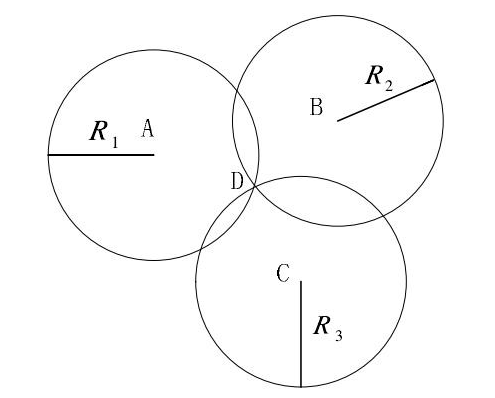
\includegraphics[width=0.7\columnwidth]{1}
\caption{Schematic diagram of the Trilateration Algorithm}
\label{fig:universe}
\end{figure}

Assume that there are n nodes randomly distributed in the wireless sensor network, and their location information is known: $(x_{1}, y_{1})(x_{2}, y_{2})(x_{3}, y_{3}) … (x_{n}, y_{n})$. Assume that the location information of the target node is X $(x_{T1}, y_{T1})$. So, the distance from the target node to each known node is:

\begin{equation*} d_{i}=\sqrt{(x_{T1}-x_{i})^{2}+(y_{T1}-y_{i})^{2}} \tag{1} \end{equation*}

Take the known node as the center and the radius from the known node to the target node as the radius. In theory, the intersection of the three circles is the coordinates of the target far point.

The Trilateration Algorithm formula is:

\begin{equation*} \begin{cases} (x_{T1}-x_{A})^{2}+(y_{T1}-y_{A})^{2}=d_{A}^{2}\\ (x_{T1}-x_{B})^{2}+(y_{T1}-y_{B})^{2}=d_{B}^{2}\\ (x_{T1}-x_{C})^{2}+(y_{T1}-y_{C})^{2}=d_{C}^{2} \end{cases} \tag{2} \end{equation*}

Through the transformation of the above formula, the coordinate information of the target node can be directly obtained as X $(x_{T1}, y_{T1})$:

\begin{equation} \begin{split} \begin{bmatrix} x_{T1}\\ y_{T1} \end{bmatrix}=\begin{bmatrix} 2(x_{A} -x_{C}) & 2(y_{A} -y_{C})\\ 2(x_{B}-x_{C}) & 2(y_{B}-y_{C}) \end{bmatrix}^{-1}
\\
\begin{bmatrix} x^{2}_{A}-x^{2}_{C}+y_{A}^{2}-y_{C}^{2}+d^{2}_{C}-d^{2}_{A}\\ x^{2}_{B}-x^{2}_{C}+y_{B}^{2}-y_{C}^{2}+d^{2}_{C}-d^{2}_{B} \end{bmatrix} \end{split} \tag{3}  \end{equation}


\subsubsection{Weighted Trilateration Algorithm}
However, in actual measurement, the three circles do not intersect at one point due to the measurement error, but intersect in a region. As a result, the Weighted Trilateration Algorithm is raised, as shown in the following Figure 2. 

\begin{figure}[!h]
\centering
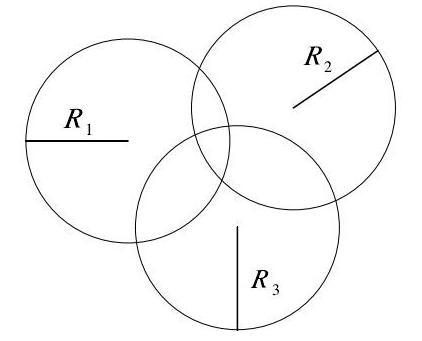
\includegraphics[width=0.6\columnwidth]{2}
\caption{Schematic diagram of the Weighted Trilateration Algorithm}
\label{fig:universe}
\end{figure}

Then add a weight $w$ and an $\beta$ to Equation (2). so that we get the unique X $(x_{T2}, y_{T2})$. To make this wand $\beta$ fit a variety of situations, use the Minimum Generalized Error method to optimize $w$ and $\beta$. By changing the values of wand $\beta$, the value of the unique target node X $(x_{T2}, y_{T2})$ is obtained.

\begin{equation*} \begin{cases} (x_{T2}-x_{A})^{2}+(y_{T2}-y_{A})^{2}=w_{A}d_{A}^{2}+\beta_{A}\\ (x_{T2}-x_{B})^{2}+(y_{T2}-y_{B})^{2}=w_{B}d_{B}^{2}+\beta_{B}\\ (x_{T2}-x_{C})^{2}+(y_{T2}-y_{C})^{2}=w_{C}d_{C}^{2}+\beta_{C} \end{cases} \tag{4} \end{equation*}

\subsection{Summary}
While there has been much research on comparison between different technologies, few researchers have taken algorithms into consideration. 
In this research, I use an RSSI-based algorithm as the method because it is simple to obtain the RSSI data from iBeacon by phone devices.

With the researcher's full understanding in the algorithms and strong capability in writing executable programs to test the function and performance of the algorithms, this research own its feasibility.

\section{Problem Statement}

\subsection{Research Problems}
The Bluetooth positioning system estimates the distance between the target and the node through RSSI, and then calculates the position of the target. However, it is a big error to estimate the distance between the target and the node through RSSI. The previous literature shows that the main reasons are:

1). The underlying protocol of Bluetooth will automatically adjust the transmit power according to the needs.

2). The multipath effect exists in the indoor environment. \cite{liu2007survey}.

\begin{figure}[!h]
\centering
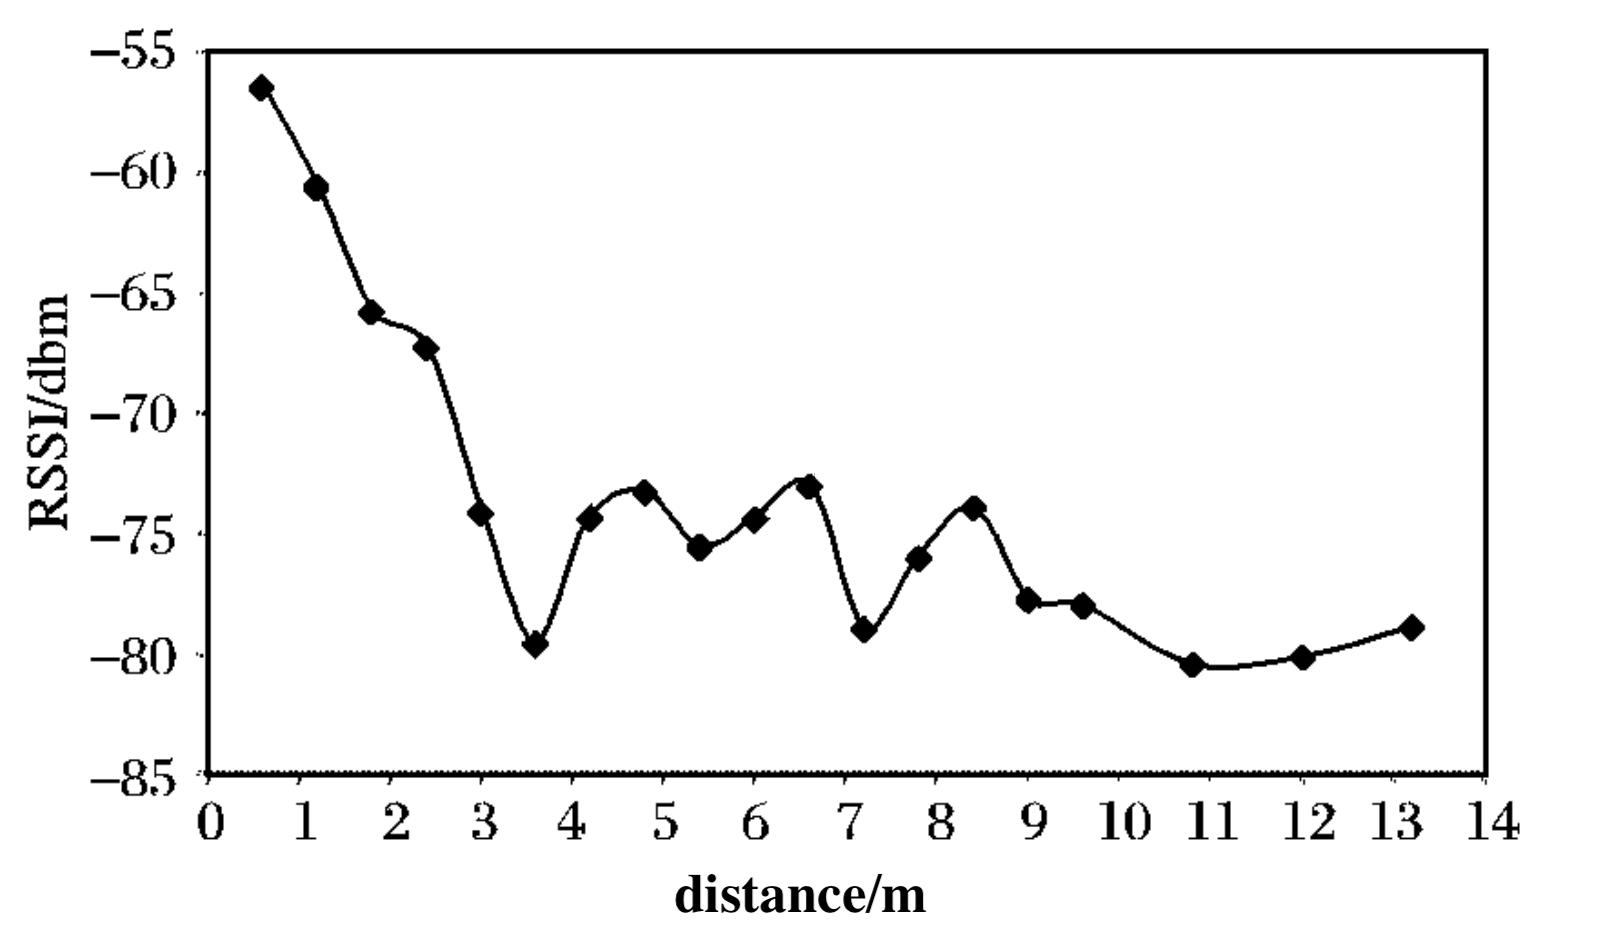
\includegraphics[width=1\columnwidth]{3.png}
\caption{Relationship between RSSI and distance}
\label{fig:universe}
\end{figure}


The measured relationship between the RSSI and the distance of the Bluetooth signal is shown in Figure 3. When the distance between the target and the node exceeds a certain range, the signal strength no longer decreases monotonically with the distance.

Thus, it is of significant important to deal with the problem with effective algorithms. When having solved this problem, the indoor positioning will become more accurate.

\subsection{Research questions}

As the accuracy of indoor position has some problems, my research questions will be addressed: What algorithm can be used to improve the accuracy of indoor positioning?

By reading numbers of literature, I find that some algorithms need to be done to filter the incorrect RSSI and the Trilateration Algorithm and the Weighted Trilateration Algorithm may be the best solution, Taking the two main algorithms into consideration, I put forward a hypothesis that compared with the Trilateration Algorithm, the Weighted Trilateration Algorithm can improve the accuracy of indoor positioning.

\subsection{Aims and Objectives}

The aim of this research is to test whether the Weighted Trilateration Algorithm is better than the Trilateration Algorithm.
Quantitative methods will be used to gain in-depth insight into the accuracy of indoor positioning based on iBeacon. This data will be analyzed and presented in the form of charts.

\section{Motivation}
 I used to develop an application that can push advertisements when a customer arrives at a store for a mall. It also used the technology of indoor positioning based on iBeacon. However, the effect is not very satisfactory due to the fluctuation of signal.
 
 Now, I want to further study the technologies and algorithms of indoor positioning to improve accuracy and stability so that it can be used in the next applications. Moreover, with the rapid increase of data services and multimedia services, the demand for positioning and navigation is increasing. I want to study deeply in this field and make my own contribution.
 
\section{Methodology}

\subsection{Research Design}

I choose quantitative methods to conduct my experiments. First of all, two different algorithms need to convert into executable code so that they can be applied in the real experiments. I will develop a wechat mini program to test the result as it can provide the ability to use Bluetooth and can receive the RSSI from the iBeacon. Then, I will deploy some iBeacons in the lab area. After that, I will use some phones with different codes to test the RSSI of each iBeacon.

That means the different algorithms are the independent variables, and the result of RSSI values are the independent variables. Extraneous variables are the lab space, the iBeacons, and the phone. All of them need to be the same.

\subsection{Data Collection}
The first stage is the signals collection. The wechat mini program collects the RSSI from deployed iBeacons. When testing the experiments, the values of RSSI will report to the server in the form of an HTTP API every second. The server program is written in the Java language. All the data are stored in the MySQL database in the form of key-value.

\subsection{Data Analysis}
After getting the experiment data, what to do next is analyzing the data.
To test and compare the performances of the given two algorithms, the accuracy (ACC) is adopted for evaluating the results. An accurate classifier will have a higher ACC value. As is shown in the following formula, the value of ACC is the sum of correct predictions divided by total predictions.

\begin{equation*} ACC(\%)=\frac{\text{Correct}\ \text{Predictions}}{\text{Total}\ \text{Predictions}}\% \tag{7} \end{equation*}

Moreover, some line charts and scatter plots are also used to summarize and demonstrate the data analysis results.

\section{Excepted Outcomes and Contributions}

\subsection{Outcomes and Limitations}
I predict that the Weighted Trilateration Algorithm will get better stability and accuracy. However, there can be a different result that the Weighted Trilateration Algorithm is not as good as the Trilateration Algorithm.

Firstly, due to the limitation of iBeacon, I can only test one kind of iBeacon which can be sold in the market. More experiments need to be conducted by test different bands of iBeacon.

Secondly, due to the limitation of phone devices, other devices may get different RSSI values. For further consideration, I will work on other experiments through different devices.

Thirdly, from the energy consumption point of view, we have discovered that the HTTP protocol over WIFI, even if simple to use, is not the best choice when a continuous communication is required since it is characterized by a very low energy efficiency. To reduce the impact on battery life, I will work on a new solution that does not rely on the HTTP protocol.

\subsection{Contributions}
In this paper, I aim to bridge the gap between the recent development in this area and the existing related survey by presenting a comparative survey of indoor positioning technologies and algorithms. Contributions in this research can be summarized as follows:

1). I provide updated research on existing indoor positioning technologies and algorithms that I believe would spur further exploration by the research community of this difficult problem area.

2). I provide a comparative analysis of indoor positioning technologies and algorithms to help indoor positioning developers in choosing the appropriate algorithms for their applications.

% Balancing columns in a ref list is a bit of a pain because you
% either use a hack like flushend or balance, or manually insert
% a column break.  http://www.tex.ac.uk/cgi-bin/texfaq2html?label=balance
% multicols doesn't work because we're already in two-column mode,
% and flushend isn't awesome, so I choose balance.  See this
% for more info: http://cs.brown.edu/system/software/latex/doc/balance.pdf
%
% Note that in a perfect world balance wants to be in the first
% column of the last page.
%
% If balance doesn't work for you, you can remove that and
% hard-code a column break into the bbl file right before you
% submit:
%
% http://stackoverflow.com/questions/2149854/how-to-manually-equalize-columns-
% in-an-ieee-paper-if-using-bibtex
%
% Or, just remove \balance and give up on balancing the last page.
%
\balance

% REFERENCES FORMAT
% References must be the same font size as other body text.

% REFERENCES FORMAT
% References must be the same font size as other body text.

% \bibliographystyle{acm-sigchi}
\bibliographystyle{unsrt}
\bibliography{sample}
\end{document}
